\section{The time-harmonic elastic wave equation at multiple frequencies}
\label{sec:EWE}
In this section we present a finite element discretization of the time-harmonic elastic wave equation with a special emphasis on the mathematical and numerical treatment when multiple frequencies (and possibly multiple right-hand sides) are present.

\subsection{Problem description}
 The time-harmonic elastic wave equation describes the displacement vector $\mathbf{u}:\Omega \rightarrow \mathbb{C}^d$ in a computational domain $\Omega \subset \mathbb{R}^{d}, d \in \{2,3\},$ governed by the following partial differential equation (PDE),
 \begin{align}
 \label{LEWE}
 -\shift_k^2 \rho(\mathbf{x}) \mathbf{u}_k - \nabla \! \cdot \! \sigma(\mathbf{u}_k) = \source , \ \mathbf{x} \in \Omega \subset \mathbb{R}^{d}, \ k=1,...,\Nom.
\end{align}

Here, $\rho(\mathbf{x})$ is the density of an elastic material in the considered domain $\Omega$ that can differ with $\mathbf{x} \in \Omega$ (inhomogeneity), $\source$ is a source term, and $\{\shift_1,...,\shift_\Nom\}$ are multiple angular frequencies that define $\Nom$ problems in \eqref{LEWE}. The stress and strain tensor follow from Hooke's law for isotropic elastic media,
\begin{align}
\label{eq:Hook}
 \sigma(\mathbf{u}_k) &:= \lambda(\mathbf{x}) \left( \nabla \! \cdot \! \mathbf{u}_k \ I_d \right) + 2 \mu(\mathbf{x}) \epsilon(\mathbf{u}_k), \\
 \epsilon(\mathbf{u}_k) &:= \frac{1}{2} \left( \nabla \mathbf{u}_k + \left( \nabla \mathbf{u}_k\right)^\mathsf{T} \right),
\end{align}
  with $\lambda, \mu$ being the Lam\'e parameters \eqref{eq:lame}. On the boundary $\partial \! \Omega$ of the domain $\Omega$, we consider the following boundary conditions,
\begin{align}
i \shift_k \rho(\mathbf{x}) B \mathbf{u}_k + \sigma(\mathbf{u}_k)\mathbf{\hat n} = \mathbf{0}, \quad \mathbf{x} \in \partial \! \Omega_a, \label{bc1}\\
\sigma(\mathbf{u}_k)\mathbf{\hat n} = \mathbf{0}, \quad \mathbf{x} \in \partial \! \Omega_r, \label{bc2}
\end{align}
where Sommerfeld radiation boundary conditions at $\partial \! \Omega_a$ model absorption, and we typically prescribe a free-surface bound\-a\-ry condition in the north of the computational domain $\partial \! \Omega_r$, with $\partial \! \Omega_a \cupdot \partial \! \Omega_r = \partial \! \Omega$. In \eqref{bc1}, $B$ is a $d \times d$ matrix that depends on $c_p$ and $c_s$, $\quad B \equiv B(\mathbf{x}) := c_p(\mathbf{x}) \mathbf{\hat n} \mathbf{\hat n}^\mathsf{T} + c_s(\mathbf{x}) \mathbf{\hat t} \mathbf{\hat t}^\mathsf{T} + c_s(\mathbf{x}) \mathbf{\hat s} \mathbf{\hat s}^\mathsf{T}$, with vectors $\{\mathbf{\hat n},\mathbf{\hat t},\mathbf{\hat s}\}$ being normal or tangential to the bound\-a\-ry, respectively; cf. \cite{apt09} for more details. Note that the boundary conditions \eqref{bc1}-\eqref{bc2} can naturally be included in a finite element approach as explained in Section \ref{ch:discretization}.
\begin{figure}[ht]
\centering
\vspace{-0.3cm}
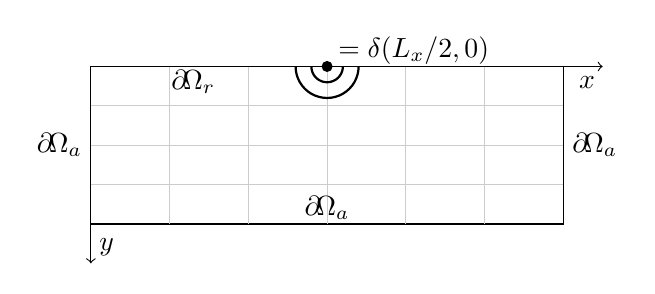
\begin{tikzpicture}
 \draw (0,0) -- (6,0) -- (6,2) -- (0,2) -- (0,0);
%  \draw (0,1) -- (4,1);
%  \draw (0,2) -- (4,2);
%  \draw (1,0) -- (1,3);
%  \draw (2,0) -- (2,3);
%  \draw (3,0) -- (3,3);

  \draw[gray!40] (0,0.5) -- (6,0.5);
  \draw[gray!40] (0,1) -- (6,1);
  \draw[gray!40] (0,1.5) -- (6,1.5);
  
  \draw[gray!40] (1,0) -- (1,2);
  \draw[gray!40] (2,0) -- (2,2);
  \draw[gray!40] (3,0) -- (3,2);
  \draw[gray!40] (4,0) -- (4,2);
  \draw[gray!40] (5,0) -- (5,2);
 
 \draw[->] (0,2) -- (6.5,2);
 \node at (6.3,1.8) {$x$};
 \draw[->] (0,2) -- (0,-0.5);
 \node at (0.2,-0.3) {$y$};
 
 \draw [thick,domain=180:360] plot ({3+0.2*cos(\x)}, {2+0.2*sin(\x)});
 \draw [thick,domain=180:360] plot ({3+0.4*cos(\x)}, {2+0.4*sin(\x)});
 \fill (3,2) circle[radius=2pt];
 
%  \fill (0,0) circle[radius=2pt];
%  \fill (1,0) circle[radius=2pt];
%  \fill (2,0) circle[radius=2pt];
%  \fill (3,0) circle[radius=2pt];
%  \fill (4,0) circle[radius=2pt];
%  \fill (0,1) circle[radius=2pt];
%  \fill (1,1) circle[radius=2pt];
%  \fill (2,1) circle[radius=2pt];
%  \fill (3,1) circle[radius=2pt];
%  \fill (4,1) circle[radius=2pt];
%  \fill (0,2) circle[radius=2pt];
%  \fill (1,2) circle[radius=2pt];
%  \fill (2,2) circle[radius=2pt];
%  \fill (3,2) circle[radius=2pt];
%  \fill (4,2) circle[radius=2pt];
%  \fill (0,3) circle[radius=2pt];
%  \fill (1,3) circle[radius=2pt];
%  \fill (3,3) circle[radius=2pt];
%  \fill (4,3) circle[radius=2pt];

 \node at (-0.4,1) {$\partial \! \Omega_a$};
 \node at (6.4,1) {$\partial \! \Omega_a$};
 \node at (3,0.2) {$\partial \! \Omega_a$};
 \node at (1.3,1.8) {$\partial \! \Omega_r$};
 
 \node at (4.1,2.2) {$\source = \boldsymbol{\delta}(L_x/2,0)$}; 
\end{tikzpicture}
\caption{Boundary conditions and source term for $d=2$. For $d=3$, the source is for instance located at $(L_x/2,L_y/2,0)^\mathsf{T}$.} \label{mesh}
\end{figure}

We assume the set of five parameters $\{\rho, c_p, c_s, \lambda, \mu\}$ in \eqref{LEWE}-\eqref{bc2} to be space-dependent. The Lam\'e parameters $\lambda$ and $\mu$ are directly related to the material density $\rho$ and the speed of P-waves $c_p$ and speed of S-waves $c_s$ via,
\begin{align}
\label{eq:lame}
%   \mu = c_s^2  \rho, \quad \lambda = c_p^2 \rho - 2 \mu.% \quad \text{ in } \Omega.
  \mu = c_s^2  \rho, \quad \lambda = \rho(c_p^2 - 2 c_s^2).% \quad \text{ in } \Omega.
\end{align}
All parameter functions are assumed in $L^1(\Omega)$. More specifically, we interpolate data points using $Q_1$ basis functions. 
\subsection{Finite element (FEM) discretization}
\label{ch:discretization}
For the discretization of \eqref{LEWE}-\eqref{bc2} we follow a classical finite element approach using the following ansatz,
\begin{align}
\label{eq:ansatz}
\mathbf{u}_k(\mathbf{x}) \approx \sum_{i=1}^\n u_k^i\boldsymbol\varphi_i(\mathbf{x}), \quad \mathbf{x} \in \Omega \subset \mathbb{R}^{d}, \quad u_k^i \in \C.
\end{align}
In the numerical examples presented in Section \ref{ch:num} we restrict ourselves to Cartesian grids and basis functions $\boldsymbol\varphi_i$ that are B-splines of degree $p$ as described for instance in \cite[Chapter 2]{isoa09}. The number of degrees of freedom is, hence, given by 
\begin{align}
\label{eq:unknows}
\n = d \prod_{i \in \{x,y,z\}} (n_i-1+p), \quad d \in \{2,3\}, p \in \mathbb{N}^{+},
\end{align}
with $n_i$ grid points in the respective spatial direction (in Figure \ref{mesh} we illustrate the case where $d=2$ and $n_x=7, n_y=5$).

\begin{definition}[Tensor notation, \cite{elman2014finite}]
\label{def:inner}
 The \textit{dot product} between two vector-valued quantities $\mathbf{u} = (u_x,u_y), \mathbf{v} = (v_x,v_y)$ is denoted as,
  $\mathbf{u} \cdot \mathbf{v} := u_x v_x + u_y v_y$. Similarly, we define the \textit{componentwise multiplication} of two matrices $U = [u_{ij}], V = [v_{ij}]$ as,
  $U : V := \sum_{i,j} u_{ij}v_{ij}$.
 \end{definition}

A Galerkin finite element approach applied to \eqref{LEWE} yields the following weak form: Find $\boldsymbol \varphi_i \in [H^1(\Omega)]^d$  such that,
\begin{align*}
% -\shift_k^2 \int_\Omega \rho(\mathbf{x}) \left(\sum_i u_k^i\boldsymbol\varphi_i\right) \boldsymbol\varphi_j \ d \! \Omega  - \int_\Omega \nabla \cdot \sigma(\sum_i u_k^i\boldsymbol\varphi_i) \boldsymbol\varphi_j \ d \! \Omega \\ = \int_\Omega \mathbf{s}  \boldsymbol\varphi_j \ d \! \Omega, \quad j=1,...,N, \\
-\shift_k^2 \sum_{i=1}^N u_k^i \int_{\Omega} \rho(\mathbf{x}) \boldsymbol\varphi_i \cdot \boldsymbol\varphi_j \ d \!\Omega - \sum_{i=1}^N u_k^i \int_\Omega \nabla \! \cdot \! \sigma(\boldsymbol\varphi_i) \cdot \boldsymbol{\varphi_j} \ d \! \Omega  \\ = \int_\Omega \source \cdot \boldsymbol\varphi_j \ d \! \Omega, \quad \text{for all }  \boldsymbol \varphi_j \in [H^1(\Omega)]^d,
\end{align*}
$j=1,...,N$, and for all source functions $\mathbf{s} \in [L^1(\Omega)]^d$. We exploit the boundary conditions \eqref{bc1}-\eqref{bc2} in the following way,
\begin{align*}
 \int_\Omega \nabla \! \cdot \! \sigma(\boldsymbol\varphi_i) \cdot \boldsymbol{\varphi_j} \ d \! \Omega \\ =  \int_{\partial \! \Omega} \sigma(\boldsymbol\varphi_i) \boldsymbol\varphi_j \cdot \mathbf{\hat n} \ d \! \Gamma - \int_\Omega \sigma(\boldsymbol\varphi_i) : \nabla \boldsymbol\varphi_j \ d \! \Omega \\
 = -i \shift_k \int_{\partial \! \Omega_a} \rho(\mathbf{x})B \boldsymbol\varphi_i \cdot \boldsymbol\varphi_j \ d \! \Gamma - \int_\Omega \sigma(\boldsymbol\varphi_i) : \nabla \boldsymbol\varphi_j \ d \! \Omega
\end{align*}
Note that the stress-free boundary condition \eqref{bc2} can be included naturally in a finite element discretization by excluding $\partial \! \Omega_r$ from the above boundary integral.
% \begin{definition}[$L^2$ inner product, \cite{elman2014finite}]
% \label{def:L2}
%  The $L^2(\Omega)$ inner product of two vector-valued functions $\mathbf{u} = (u_x,u_y), \mathbf{v} = (v_x,v_y)$ is defined as
%  \begin{align*}
%   \left\langle \mathbf{u} , \mathbf{v} \right\rangle_{L^2(\Omega)} := \int_\Omega \mathbf{u}^\trp \mathbf{v} \ d \! \Omega =  \int_\Omega (u_x v_x + u_y v_y) \ d \! \Omega.
%  \end{align*}
% \end{definition}

We summarize the finite element discretization of the time-harmonic, inhomogeneous elastic wave equation at multiple frequencies $\shift_k$ by,
\begin{align}
\label{eq:disc_prob}
 (K + i \shift_k C - \shift_k^2 M) \x_k = \rhs, \quad k = 1,...,\Nom, %\ \{K,C,M\} \in \mathbb{R}^{N \times N},
\end{align}
with unknown vectors $\x_k := [u_k^1,...,u_k^N]^\mathsf{T} \in \C^\n$ consisting of the coefficients in \eqref{eq:ansatz}, and mass matrix $M$, stiffness matrix $K$ and boundary matrix $C$ given by,
\begin{alignat*}{3}
 & [K]_{ij} &&= \int_\Omega \sigma(\boldsymbol\varphi_i) : \nabla \boldsymbol\varphi_j \ d \! \Omega, \quad 
 [M]_{ij} &&= \int_\Omega \rho \boldsymbol\varphi_i \cdot \boldsymbol\varphi_j \ d \! \Omega, \\
 & [C]_{ij} &&= \int_{\partial \! \Omega_a} \rho B \boldsymbol\varphi_i \cdot \boldsymbol\varphi_j \ d \! \Gamma, \quad \phantom{aa}
 [\mathbf{b}]_j &&= \int_\Omega \source \cdot \boldsymbol\varphi_j \ d \! \Omega.
%  K_{ij} &= \int_\Omega \sigma(\boldsymbol\varphi_i) : \nabla \boldsymbol\varphi_j \ d \! \Omega, \\ %\quad \sigma(\boldsymbol\varphi_i) := \lambda(\mathbf{x}) \text{div}(\boldsymbol\varphi_i) I_d + \mu(\mathbf{x}) \left( \nabla \boldsymbol\varphi_i + (\nabla \boldsymbol\varphi_i)^\mathsf{T}\right),\\
%  C_{ij} &= \left\langle \rho(\mathbf{x}) B \boldsymbol\varphi_i , \boldsymbol\varphi_j \right\rangle_{L^2(\partial \! \Omega_a)} \equiv \int_{\partial \! \Omega_a} \rho(\mathbf{x}) B \boldsymbol\varphi_i^\trp \boldsymbol\varphi_j \ d \! \Gamma, \\ %\quad B := c_p(\mathbf{x}) \mathbf{\hat n} \mathbf{\hat n}^\mathsf{T} + c_s(\mathbf{x}) \mathbf{\hat t} \mathbf{\hat t}^\mathsf{T} + c_s(\mathbf{x}) \mathbf{\hat s} \mathbf{\hat s}^\mathsf{T},\\
%  M_{ij} &= \left\langle \rho(\mathbf{x}) \boldsymbol\varphi_i , \boldsymbol\varphi_j \right\rangle_{L^2(\Omega)} \equiv \int_\Omega \rho(\mathbf{x}) \boldsymbol\varphi_i^\trp \boldsymbol\varphi_j \ d \! \Omega.
\end{alignat*}
In a 2D problem (see Figure \ref{mesh}), the unknown $\x_k$ contains the $x$-components and the $y$-components of the displacement vector. When lexicographic numbering is used, the matrices in \eqref{eq:disc_prob} have the block structure
\begin{align*}
 K = \begin{bmatrix}
      K_{xx} & K_{xy} \\ K_{yx} & K_{yy}
     \end{bmatrix}, \quad
 C = \begin{bmatrix}
      C_{xx} & C_{xy} \\ C_{yx} & C_{yy}
     \end{bmatrix}, \quad
 M = \begin{bmatrix}
      M_{xx} & M_{xy} \\ M_{yx} & M_{yy}
     \end{bmatrix},
\end{align*}
as shown in Figure \ref{fig:perm} (left) for $d=2$, and Figure \ref{fig:hier_struc} (top left) for $d=3$. When solving \eqref{eq:disc_prob} with an iterative Krylov method, it is necessary to apply a preconditioner. Throughout this document, we consider a preconditioner of the form
\begin{equation}
 \label{eq:precon}
 \mathcal{P}(\tau) = (K + i \tau C - \tau^2M),
\end{equation}
where $\tau$ is a single \textit{seed frequency} that needs to be chosen with care for the range of frequencies $\{ \omega_1,...\omega_\Nom\}$, cf. the considerations in \cite{BG15,SBK13}. The efficient application of the preconditioner \eqref{eq:precon} for problems of dimension $d=2$ and $d=3$ on a structured domain is presented in Section \ref{ch:msss}, and the choice of $\tau$ is discussed in Section \ref{ch:best_tau}.

\begin{figure}[H]
\centering
%   \includegraphics[width=0.4\columnwidth]{figs/13-06-52/P-crop.pdf} \hspace{0.5cm} %{figs/P31-crop.pdf} \hspace{0.5cm}
%   \includegraphics[width=0.4\columnwidth]{figs/13-06-52/P3D_orig-crop.pdf} \\ \vspace{0.5cm} %{figs/P31_x-crop.pdf} \\ \vspace{0.5cm}
%   \includegraphics[width=0.4\columnwidth]{figs/13-06-52/P2D_orig-crop.pdf} \hspace{0.5cm} %{figs/P31_xx-crop.pdf} \hspace{0.5cm}
%   \includegraphics[width=0.4\columnwidth]{figs/13-06-52/P1D_orig-crop.pdf} %{figs/P31_xx-crop.pdf} 
  \includegraphics[width=\columnwidth]{3d_hier_matrix.pdf}
\caption{A \texttt{spy} plot of \eqref{eq:precon} for a 3D elastic problem when linear basis functions ($p=1$) are used: In the top row we show the discretized problem for lexicographic (top left) and nodal-based ordering (top right). Appropriate zooming demonstrates the hierarchically repeating structure of the matrix on level 2 (bottom left) and level 1 (bottom right). For level~1, we indicate the SSS data structure used in Section \ref{ch:sss_level1}. Here, the rank of $U_2$ equals one.}
\label{fig:hier_struc}
\end{figure}
\subsection{Reformulation as a matrix equation}
We next describe a new approach to solve \eqref{eq:disc_prob} at multiple frequencies. Therefore, we define the block matrix $\X$ consisting of all unknown vectors, $\X := [\x_1,...,\x_\Nom] \in \mathbb{C}^{\n \times \Nom}$, and note that \eqref{eq:disc_prob} can be rewritten as,
\begin{align}
\label{eq:mateq_approach2}
\op(\X) := K \X + i C \X \Sigma - M \X \Sigma^2 = \blkrhs,
\end{align}
where $\Sigma := \text{diag}(\omega_1,...,\omega_{\Nom})$, and with block right-hand side $\blkrhs := [\rhs,...,\rhs]$.
In \eqref{eq:mateq_approach2}, we also define the linear operator $\op(\cdot)$
which defines the matrix equation \eqref{eq:mateq_approach2} in short-hand notation as $\op(\X) =
\blkrhs$. This reformulation gives rise to use an extension of the IDR($s$) method
to solve linear matrix equations \cite{ag15}.\\

Note that an alternative approach to efficiently solve \eqref{eq:disc_prob} at multiple frequencies ($\Nom > 1$) leads to the solution of shifted linear systems as presented in \cite[Section 4.2]{BG15} and the references therein. The memory-efficient approach followed by \cite{BG15} relies on the shift-invariance property of the Krylov spaces belonging to different frequencies. Some restrictions of this approach like collinear right-hand sides in \eqref{eq:disc_prob} and the difficulty of preconditioner design are, however, not present in the matrix equation setting \eqref{eq:mateq_approach2}. 
